\documentclass{article}
\usepackage[utf8]{inputenc}

%\usepackage[md]{titlesec}
\usepackage{graphicx}

\usepackage[export]{adjustbox}
\usepackage{color}
\usepackage{hyperref} %% Enable hyperref links from toc
\hypersetup{
    colorlinks,
    citecolor=black,
    filecolor=black,
    linkcolor=blue,
    urlcolor=black
}

\usepackage{subcaption} % Enables subcaption

% Sets the depth of toc to be limited to sections
\setcounter{tocdepth}{2} 

%% Changes the subsection to be numbered with alphabets
\renewcommand{\thesubsection}{\alph{subsection}}
%\renewcommand{\thesubsubsection}{\arabic{\subsubsection}}



\date{October 24, 2016}


\title{\textbf{Assignment 9}\\Practical tasks in the networking Lab}
\author{Siddhartha Pandey (s316620)\\
\textit{Worked with}:\\ Mathias J.P. Stang (s316623)\\
Samiul Saki Chowdhury (s316611)
}

\begin{document}

\maketitle
\newpage
\tableofcontents
\newpage



For this assignment we used one router(\textit{cisco 2800}), one switch (\textit{catalyst 2900}) and two hosts ( one running Ubuntu 14.04 and another Mac OS X).

\section{Console access to a real router}

\begin{figure}[h]
    \centering
    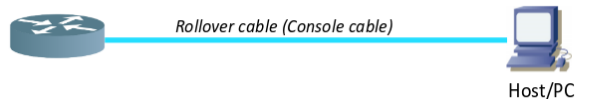
\includegraphics[width=0.8\textwidth]{1topo}
    \caption{Topology from Figure 1 in Assignment 9}
    \label{fig:1topo}
\end{figure}

\subsection{Connecting the host and the router}
We now connect the \textit{Ubuntu host} to the router. The cable was connected to the consolse port on the router, the cable used was a RJ45-DB9 Cisco console cable. Our topology can be seen in Figure \ref{fig:1topo}. The \textit{minicom} program was used to communicate with the router by running the \textbf{minicom cisco1} command on the Ubuntu host terminal. The minicom configurations were stored from before in the \textit{cisco1} file at Ubuntu host.  The \textit{minicom} program gives us the Command Line Interface (CLI) for the router. 

\subsection{Using the CLI}
At the start of the CLI we were in the user mode. We issued the same commands as we did in the PacketTracer in the first part of Assignment7. We issued the following commands respectively : 
\begin{itemize}
    \item \textbf{enable} Go to the privileged mode (enable mode).
    \item \textbf{configure terminal} Go to the configure mode.
    \item \textbf{hostname MyRouter} Changed the hostname to 'MyRouter', this was done in configure mode. 
    \item \textbf{write} Save the changes persistently across reboots. This command was issued in the enable mode. 
\end{itemize}

The only difference we noticed was the the physical router took more time compared to the virtual router in Packet Tracer. 


\section{Connecting two real hosts to a real router}

\begin{figure}[h]
    \centering
    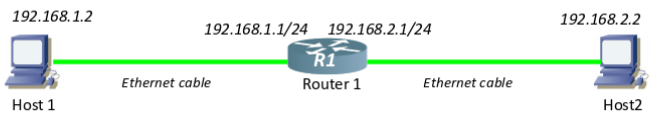
\includegraphics[width=0.8\textwidth]{2topo}
    \caption{Topology from Figure 2 in Assignment 9}
    \label{fig:2topo}
\end{figure}

Now we modify our topology by connecting two hosts to the router as seen in Figure \ref{fig:2topo}. The two hosts were connected to the router using an Ethernet cable.
The hosts were configure as per the specification from Figure \ref{fig:2topo}, Host1 is the host running the Mac OSx and Host2 is the Ubuntu Host.  

\subsection{Configuring the router}
We setup the IP addresses for the interfaces connected to the two hosts in the router and made sure they were \textit{up}. We ran the following commands:
\begin{verbatim}
    MyRouter>enable
    MyRouter#conf t
    MyRouter(config)#interface Fa0/0
    MyRouter(config-if)#ip address 192.168.1.1 255.255.255.0
    MyRouter(config-if)#no shutdown
    MyRouter(config-if)#exit
    MyRouter(config)#interface Fa0/1
    MyRouter(config-if)#ip address 192.168.2.1 255.255.255.0
    MyRouter(config-if)#no shutdown 
\end{verbatim}

\subsection{Configuring the hosts}

We then configured the hosts by setting up the interfaces with IP addresses and made sure they were \textit{up}. There were two interfaces in the Ubuntu host ( \textit{enp0s25} and \textit{enp4s2}), we figured out which one was connected to the router by running the command \textbf{ifconfig enp0s25 down} this stoped the light on the port that was connected to the router from blinking, confirming that \textit{enp0s25} was the interface connected to the router. While on the Host1 (OSx host) we figured this with trial and error method. We used the following commands to configure the IP addresses to the hosts:
\begin{verbatim}
    ifconfig <interface> <IP addresss>/<subnet prefix>
\end{verbatim}
Where the \textit{interface} was the interface name on the particular hosts, the \textit{IP address} was the IP address for that interface and the \textit{subnet prefix} was the prefix for the subnet. We had some problems with configuring the IP address for the Ubuntu host as it would automatically remove the IP address from time to time, when some commands were run in the router regarding the interface that the host was connected to or if the cable was disconnected and connected again. We also configured the default gateway on the hosts to the IP address of the interface of the router to which the hosts were connected by using the command \textbf{route add default gw \textless\textit{IP address}\textgreater \textless\textit{interface}\textgreater} where the \textit{IP address} is the IP address of the router's interface where the host was connected and the \textit{interface} is the interface name at the host. 

\subsection{Checking connectivity}

To check the connectivity we ran the \textbf{ping} command from the hosts. Initially we could ping from Host1 (192.168.1.2, running OSx) to the both the interface of the router(192.168.1.1 and 192.168.2.1) and Ubuntu host (192.168.2.2). But pinging from the router and Ubuntu host to Host1 we did not get connectivity, this problem was solved after the firewall was disabled on Host1 and the IP address was set from the GUI. When the GUI was opened the IP address of the interface connected to the router was 192.168.1.10, it was changed to 192.168.1.2 to make the ping command work. The connectivity from Host1(192.168.1.2) to Ubuntu host(192.168.2.2) can be seen in Figure \ref{fig:2ping}.

\begin{figure}[h]
    \centering
    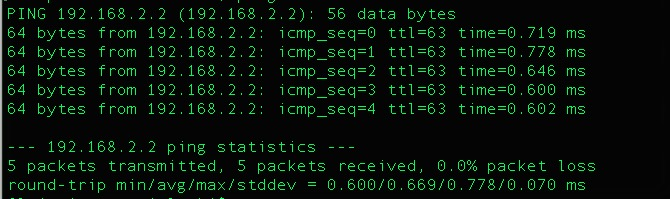
\includegraphics[width=0.8\textwidth]{2ping}
    \caption{\textbf{ping} from Host1(192.168.1.2) to Ubuntu host(192.168.2.2).}
    \label{fig:2ping}
\end{figure}


\section{Router-on-a-stick}

Then we modify our topology to look as it does in Figure \ref{fig:3topo}. We connect the two hosts to the switch and then connect the switch to the router. We also implement a VLAN with Host1(192.168.1.2) as part of VLAN 10 and Ubuntu host/Host2 (192.168.2.2) as part of VLAN 20. We configure the switch and the routers accordingly to have connectivity between hosts in the different VLANs. 

\begin{figure}[h]
    \centering
    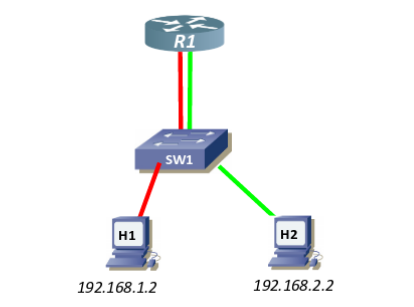
\includegraphics[width=0.5\textwidth]{3topo}
    \caption{Router-on-a-stick topology from Figure 3 in Assignment 9.}
    \label{fig:3topo}
\end{figure}

\subsection{Configuring the switch}

In the switch we add the different VLANs and the configure the ports connected to the hosts to be in the access mode, and which port should be in which vlan, and the port connected to the router to be in the trunk mode. We can see in Table \ref{tab:3portscon} the ports where the hosts and the routers were connected. 

\begin{table}[h]
    \centering
    \begin{tabular}{|c|c|}
    \hline
        Port & Connected host \\
        \hline
         Fa 0/1 & Host2 (192.168.2.2, Ubuntu)\\
         Fa 0/2 & Host1 (192.168.1.2, OsX)\\
         Fa 0/3 & Router (192.168.1.1 \& 192.168.2.1)\\
         \hline     
    \end{tabular}
    \caption{Ports connection at switch}
    \label{tab:3portscon}
\end{table}

We used the following commands to set up the switch:
\begin{verbatim}
    Switch>enable
    Switch# conf t
    Switch(config)#vlan 10
    Switch(config-vlan)#exit
    Switch(config)#vlan 20
    Switch(config-vlan)#exit
    Switch(config)#interface Fa0/1
    Switch(config-if)#switchport mode access
    Switch(config-if)#switchport access vlan 20
    Switch(config-if)#exit
    Switch(config)#interface Fa0/2
    Switch(config-if)#switchport mode access
    Switch(config-if)#switchport access vlan 10 
    Switch(config-if)#exit
    Switch(config)#interface Fa0/3
    Switch(config-if)#switchport mode trunk
    Switch(config-if)#switchport trunk allowed vlan all
    Switch(config-if)#do write
\end{verbatim}

We saved the changes persistently using the \textbf{write} command and confirmed the changes using the \textbf{show interface trunk} and \textbf{show vlan} commands.

\subsection{Configuring the router}

In the router we made sure that the interface connected to the switch was \textit{up}, then made two sub-interfaces in the interface connected to the switch. We gave IP address for each of the sub-interface and enable the sub-interface to use the IEEE 802.1Q VLAN encapsulation protocol and assign a VLAN. The commands used to do this are as follows: 

\begin{verbatim}
    Router>enable
    Router#conf t
    Router(config)#interface Fa0/1
    Router(config-if)#no shutdown
    Router(config-if)#no ip address
    Router(config-if)#exit
    Router(config)#interface Fa0/1.10
    Router(config-if)#encapsulation dot1Q 10 
    Router(config-if)#ip address 192.168.1.1 255.255.255.0
    Router(config-if)#exit
    Router(config)#interface Fa0/1.20
    Router(config-if)#encapsulation dot1Q 20 
    Router(config-if)#ip address 192.168.2.1 255.255.255.0
    Router(config-if)#exit
    Router(config)#do write
\end{verbatim}

We had connectivity between the two hosts after configuring the router and the switch. We did have a problem with Ubuntu host losing the IP address on its interface but it was solved by assigning its IP address again, as mentioned previously.

\section{VLAN(Virtual LAN) implemented on real switches}

\begin{figure}
    \centering
    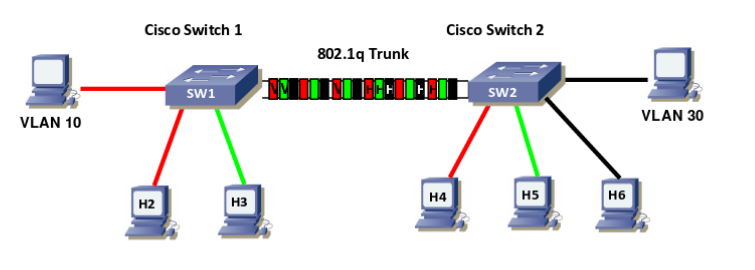
\includegraphics[width=0.9\textwidth]{4topo}
    \caption{Topology from Figure 3 in Assignment 9. Our topology looks similar with two hosts connected to the Switches and VLAN 10 and 30 connected to Switch1 and VLAN 10 and 20 connected to Switch2}
    \label{fig:4topo}
\end{figure}

We also tested VLAN implemented on two switches. We used the topology similar to Figure \ref{fig:4topo} but only had two hosts connected to each switch. Our hosts had the specifications as seen in Table \ref{tab:4topospecs}. 

\begin{table}
    \centering
    \begin{tabular}{|c|c|c|c|}
    \hline
         Switch & Host & VLAN ID & IP address\\
    \hline
    Switch1 & Host1 & 10 & 192.168.1.2 \\
    Switch1 & Host2 & 30 & 192.168.3.2 \\
    Switch2 & UbuntuHost & 20 & 192.168.2.2 \\
    Switch2 & MacOsX & 10 & 192.168.1.5 \\
    \hline
    \end{tabular}
    \caption{Topology specifications}
    \label{tab:4topospecs}
\end{table}

The switches had two hosts each and the two switches were connected to each other. The ports connecting the switches were in the trunk mode and the ports that were connected to the hosts were in access mode. This experiment was done with one other group. Our group managed Switch2 and the other group managed Switch1. Host1 and MacOsX could ping each other as they were in the same VLAN but there was no connectivity between the hosts in other VLANs. 

\section{Cleaning the Devices}

All the configurations in the devices that was implemented in this assignment was removed and restored to factory default settings. This was done using the \textbf{write erase} command in the enable mode for both the router and the switch to remove the configurations stored in the \textit{nvram}. We also deleted the VLAN configurations in the switch, as it is not in the \textit{nvram}, by running the command \textbf{delete vlan.dat}. 


\end{document}
